% Options for packages loaded elsewhere
\PassOptionsToPackage{unicode}{hyperref}
\PassOptionsToPackage{hyphens}{url}
%
\documentclass[
  man,floatsintext]{apa6}
\usepackage{amsmath,amssymb}
\usepackage{iftex}
\ifPDFTeX
  \usepackage[T1]{fontenc}
  \usepackage[utf8]{inputenc}
  \usepackage{textcomp} % provide euro and other symbols
\else % if luatex or xetex
  \usepackage{unicode-math} % this also loads fontspec
  \defaultfontfeatures{Scale=MatchLowercase}
  \defaultfontfeatures[\rmfamily]{Ligatures=TeX,Scale=1}
\fi
\usepackage{lmodern}
\ifPDFTeX\else
  % xetex/luatex font selection
\fi
% Use upquote if available, for straight quotes in verbatim environments
\IfFileExists{upquote.sty}{\usepackage{upquote}}{}
\IfFileExists{microtype.sty}{% use microtype if available
  \usepackage[]{microtype}
  \UseMicrotypeSet[protrusion]{basicmath} % disable protrusion for tt fonts
}{}
\makeatletter
\@ifundefined{KOMAClassName}{% if non-KOMA class
  \IfFileExists{parskip.sty}{%
    \usepackage{parskip}
  }{% else
    \setlength{\parindent}{0pt}
    \setlength{\parskip}{6pt plus 2pt minus 1pt}}
}{% if KOMA class
  \KOMAoptions{parskip=half}}
\makeatother
\usepackage{xcolor}
\usepackage{color}
\usepackage{fancyvrb}
\newcommand{\VerbBar}{|}
\newcommand{\VERB}{\Verb[commandchars=\\\{\}]}
\DefineVerbatimEnvironment{Highlighting}{Verbatim}{commandchars=\\\{\}}
% Add ',fontsize=\small' for more characters per line
\usepackage{framed}
\definecolor{shadecolor}{RGB}{248,248,248}
\newenvironment{Shaded}{\begin{snugshade}}{\end{snugshade}}
\newcommand{\AlertTok}[1]{\textcolor[rgb]{0.94,0.16,0.16}{#1}}
\newcommand{\AnnotationTok}[1]{\textcolor[rgb]{0.56,0.35,0.01}{\textbf{\textit{#1}}}}
\newcommand{\AttributeTok}[1]{\textcolor[rgb]{0.13,0.29,0.53}{#1}}
\newcommand{\BaseNTok}[1]{\textcolor[rgb]{0.00,0.00,0.81}{#1}}
\newcommand{\BuiltInTok}[1]{#1}
\newcommand{\CharTok}[1]{\textcolor[rgb]{0.31,0.60,0.02}{#1}}
\newcommand{\CommentTok}[1]{\textcolor[rgb]{0.56,0.35,0.01}{\textit{#1}}}
\newcommand{\CommentVarTok}[1]{\textcolor[rgb]{0.56,0.35,0.01}{\textbf{\textit{#1}}}}
\newcommand{\ConstantTok}[1]{\textcolor[rgb]{0.56,0.35,0.01}{#1}}
\newcommand{\ControlFlowTok}[1]{\textcolor[rgb]{0.13,0.29,0.53}{\textbf{#1}}}
\newcommand{\DataTypeTok}[1]{\textcolor[rgb]{0.13,0.29,0.53}{#1}}
\newcommand{\DecValTok}[1]{\textcolor[rgb]{0.00,0.00,0.81}{#1}}
\newcommand{\DocumentationTok}[1]{\textcolor[rgb]{0.56,0.35,0.01}{\textbf{\textit{#1}}}}
\newcommand{\ErrorTok}[1]{\textcolor[rgb]{0.64,0.00,0.00}{\textbf{#1}}}
\newcommand{\ExtensionTok}[1]{#1}
\newcommand{\FloatTok}[1]{\textcolor[rgb]{0.00,0.00,0.81}{#1}}
\newcommand{\FunctionTok}[1]{\textcolor[rgb]{0.13,0.29,0.53}{\textbf{#1}}}
\newcommand{\ImportTok}[1]{#1}
\newcommand{\InformationTok}[1]{\textcolor[rgb]{0.56,0.35,0.01}{\textbf{\textit{#1}}}}
\newcommand{\KeywordTok}[1]{\textcolor[rgb]{0.13,0.29,0.53}{\textbf{#1}}}
\newcommand{\NormalTok}[1]{#1}
\newcommand{\OperatorTok}[1]{\textcolor[rgb]{0.81,0.36,0.00}{\textbf{#1}}}
\newcommand{\OtherTok}[1]{\textcolor[rgb]{0.56,0.35,0.01}{#1}}
\newcommand{\PreprocessorTok}[1]{\textcolor[rgb]{0.56,0.35,0.01}{\textit{#1}}}
\newcommand{\RegionMarkerTok}[1]{#1}
\newcommand{\SpecialCharTok}[1]{\textcolor[rgb]{0.81,0.36,0.00}{\textbf{#1}}}
\newcommand{\SpecialStringTok}[1]{\textcolor[rgb]{0.31,0.60,0.02}{#1}}
\newcommand{\StringTok}[1]{\textcolor[rgb]{0.31,0.60,0.02}{#1}}
\newcommand{\VariableTok}[1]{\textcolor[rgb]{0.00,0.00,0.00}{#1}}
\newcommand{\VerbatimStringTok}[1]{\textcolor[rgb]{0.31,0.60,0.02}{#1}}
\newcommand{\WarningTok}[1]{\textcolor[rgb]{0.56,0.35,0.01}{\textbf{\textit{#1}}}}
\usepackage{graphicx}
\makeatletter
\def\maxwidth{\ifdim\Gin@nat@width>\linewidth\linewidth\else\Gin@nat@width\fi}
\def\maxheight{\ifdim\Gin@nat@height>\textheight\textheight\else\Gin@nat@height\fi}
\makeatother
% Scale images if necessary, so that they will not overflow the page
% margins by default, and it is still possible to overwrite the defaults
% using explicit options in \includegraphics[width, height, ...]{}
\setkeys{Gin}{width=\maxwidth,height=\maxheight,keepaspectratio}
% Set default figure placement to htbp
\makeatletter
\def\fps@figure{htbp}
\makeatother
\setlength{\emergencystretch}{3em} % prevent overfull lines
\providecommand{\tightlist}{%
  \setlength{\itemsep}{0pt}\setlength{\parskip}{0pt}}
\setcounter{secnumdepth}{-\maxdimen} % remove section numbering
% Make \paragraph and \subparagraph free-standing
\ifx\paragraph\undefined\else
  \let\oldparagraph\paragraph
  \renewcommand{\paragraph}[1]{\oldparagraph{#1}\mbox{}}
\fi
\ifx\subparagraph\undefined\else
  \let\oldsubparagraph\subparagraph
  \renewcommand{\subparagraph}[1]{\oldsubparagraph{#1}\mbox{}}
\fi
% definitions for citeproc citations
\NewDocumentCommand\citeproctext{}{}
\NewDocumentCommand\citeproc{mm}{%
  \begingroup\def\citeproctext{#2}\cite{#1}\endgroup}
\makeatletter
 % allow citations to break across lines
 \let\@cite@ofmt\@firstofone
 % avoid brackets around text for \cite:
 \def\@biblabel#1{}
 \def\@cite#1#2{{#1\if@tempswa , #2\fi}}
\makeatother
\newlength{\cslhangindent}
\setlength{\cslhangindent}{1.5em}
\newlength{\csllabelwidth}
\setlength{\csllabelwidth}{3em}
\newenvironment{CSLReferences}[2] % #1 hanging-indent, #2 entry-spacing
 {\begin{list}{}{%
  \setlength{\itemindent}{0pt}
  \setlength{\leftmargin}{0pt}
  \setlength{\parsep}{0pt}
  % turn on hanging indent if param 1 is 1
  \ifodd #1
   \setlength{\leftmargin}{\cslhangindent}
   \setlength{\itemindent}{-1\cslhangindent}
  \fi
  % set entry spacing
  \setlength{\itemsep}{#2\baselineskip}}}
 {\end{list}}
\usepackage{calc}
\newcommand{\CSLBlock}[1]{\hfill\break\parbox[t]{\linewidth}{\strut\ignorespaces#1\strut}}
\newcommand{\CSLLeftMargin}[1]{\parbox[t]{\csllabelwidth}{\strut#1\strut}}
\newcommand{\CSLRightInline}[1]{\parbox[t]{\linewidth - \csllabelwidth}{\strut#1\strut}}
\newcommand{\CSLIndent}[1]{\hspace{\cslhangindent}#1}
\ifLuaTeX
\usepackage[bidi=basic]{babel}
\else
\usepackage[bidi=default]{babel}
\fi
\babelprovide[main,import]{english}
% get rid of language-specific shorthands (see #6817):
\let\LanguageShortHands\languageshorthands
\def\languageshorthands#1{}
% Manuscript styling
\usepackage{upgreek}
\captionsetup{font=singlespacing,justification=justified}

% Table formatting
\usepackage{longtable}
\usepackage{lscape}
% \usepackage[counterclockwise]{rotating}   % Landscape page setup for large tables
\usepackage{multirow}		% Table styling
\usepackage{tabularx}		% Control Column width
\usepackage[flushleft]{threeparttable}	% Allows for three part tables with a specified notes section
\usepackage{threeparttablex}            % Lets threeparttable work with longtable

% Create new environments so endfloat can handle them
% \newenvironment{ltable}
%   {\begin{landscape}\centering\begin{threeparttable}}
%   {\end{threeparttable}\end{landscape}}
\newenvironment{lltable}{\begin{landscape}\centering\begin{ThreePartTable}}{\end{ThreePartTable}\end{landscape}}

% Enables adjusting longtable caption width to table width
% Solution found at http://golatex.de/longtable-mit-caption-so-breit-wie-die-tabelle-t15767.html
\makeatletter
\newcommand\LastLTentrywidth{1em}
\newlength\longtablewidth
\setlength{\longtablewidth}{1in}
\newcommand{\getlongtablewidth}{\begingroup \ifcsname LT@\roman{LT@tables}\endcsname \global\longtablewidth=0pt \renewcommand{\LT@entry}[2]{\global\advance\longtablewidth by ##2\relax\gdef\LastLTentrywidth{##2}}\@nameuse{LT@\roman{LT@tables}} \fi \endgroup}

% \setlength{\parindent}{0.5in}
% \setlength{\parskip}{0pt plus 0pt minus 0pt}

% Overwrite redefinition of paragraph and subparagraph by the default LaTeX template
% See https://github.com/crsh/papaja/issues/292
\makeatletter
\renewcommand{\paragraph}{\@startsection{paragraph}{4}{\parindent}%
  {0\baselineskip \@plus 0.2ex \@minus 0.2ex}%
  {-1em}%
  {\normalfont\normalsize\bfseries\itshape\typesectitle}}

\renewcommand{\subparagraph}[1]{\@startsection{subparagraph}{5}{1em}%
  {0\baselineskip \@plus 0.2ex \@minus 0.2ex}%
  {-\z@\relax}%
  {\normalfont\normalsize\itshape\hspace{\parindent}{#1}\textit{\addperi}}{\relax}}
\makeatother

% \usepackage{etoolbox}
\makeatletter
\patchcmd{\HyOrg@maketitle}
  {\section{\normalfont\normalsize\abstractname}}
  {\section*{\normalfont\normalsize\abstractname}}
  {}{\typeout{Failed to patch abstract.}}
\patchcmd{\HyOrg@maketitle}
  {\section{\protect\normalfont{\@title}}}
  {\section*{\protect\normalfont{\@title}}}
  {}{\typeout{Failed to patch title.}}
\makeatother

\usepackage{xpatch}
\makeatletter
\xapptocmd\appendix
  {\xapptocmd\section
    {\addcontentsline{toc}{section}{\appendixname\ifoneappendix\else~\theappendix\fi\\: #1}}
    {}{\InnerPatchFailed}%
  }
{}{\PatchFailed}
\keywords{ordinal, likert, simulations, power\newline\indent Word count: X}
\usepackage{csquotes}
\ifLuaTeX
  \usepackage{selnolig}  % disable illegal ligatures
\fi
\IfFileExists{bookmark.sty}{\usepackage{bookmark}}{\usepackage{hyperref}}
\IfFileExists{xurl.sty}{\usepackage{xurl}}{} % add URL line breaks if available
\urlstyle{same}
\hypersetup{
  pdftitle={Ordinal regression models made easy. A tutorial on parameter interpretation, data simulation, and power analysis.},
  pdfauthor={Filippo Gambarota1 \& Gianmarco Altoè1},
  pdflang={en-EN},
  pdfkeywords={ordinal, likert, simulations, power},
  hidelinks,
  pdfcreator={LaTeX via pandoc}}

\title{Ordinal regression models made easy. A tutorial on parameter interpretation, data simulation, and power analysis.}
\author{Filippo Gambarota\textsuperscript{1} \& Gianmarco Altoè\textsuperscript{1}}
\date{}


\shorttitle{Ordinal regression models made easy}

\authornote{

Add complete departmental affiliations for each author here. Each new line herein must be indented, like this line.

Enter author note here.

The authors made the following contributions. Filippo Gambarota: Conceptualization, Writing - Original Draft Preparation, Writing - Review \& Editing; Gianmarco Altoè: Writing - Review \& Editing, Supervision.

Correspondence concerning this article should be addressed to Filippo Gambarota, Postal address. E-mail: \href{mailto:filippo.gambarota@unipd.it}{\nolinkurl{filippo.gambarota@unipd.it}}

}

\affiliation{\vspace{0.5cm}\textsuperscript{1} Department of Developmental Psychology and Socialization, University of Padova, Italy}

\abstract{%
Abstract here
}



\begin{document}
\maketitle

\section{Introduction}\label{introduction}

Da citare in qualche modo Kemp and Grace (2021)

\begin{quote}
``As a matter of fact, most of the scales used widely and effectively by psychologists are ordinal scales. In the strictest propriety the ordinary statistics involving means and standard deviations ought not to be used with these scales, for these statistics imply a knowledge of something more than the relative rank-order of data. On the other hand for this `illegal' statisticizing there can be invoked a kind of pragmatic sanction: In numerous instances it leads to fruitful results.'' (Stevens, 1946, p.~679.)
\end{quote}

\begin{quote}
It is straightforward to construct ordinal scales that do not involve rank ordering. For example, one can take the first element encountered and arbitrarily assign it the number 100. If the next element encountered is smaller it is given a smaller arbitrary number, 53 say. If the third element is between these two, it can be given the number 86, and so on. If this construction method is used, the difference between the elements assigned the numbers 70 and 80 will not in any important sense be equal to the difference between the elements assigned 90 and 100, and the intervals between the numbers are not really interpretable. Note, too, that monotonic transformations of the scale essentially leave the mea- sure unaffected.
\end{quote}

interessante come Cliff (2016) descriva che la maggiorparte dellle domande di ricerca in psicologia siano in riferimento alla location di un costrutto e possano essere gestite in modo ordinale

The use of ordinal data is widespread in Psychology. Usually items from questionnaires are created using Likert scales where a certain psychological traits is measured using an intuitive scale with 3-5 or more anchor points. These measure cannot be considered \emph{metric} measure on interval or ratio scales {[}stevens{]} but the categories are ordered.

Other examples here

Despite the usage of ordinal variables, statistical models made for these type of data are rarely used in Psychology. Liddell and Kruschke (2018) reported that the majority of published papers using likert-like measures used standard methods to analyze the data. In practical terms, they use \emph{metric} models where the response variable cannot be considered fully numeric (vedi se c'è un termine tipo scala a rapporti).

altro sui modelli

Theoretically, using a \emph{metric} for ordinal data is not appropriate but understanding the actual impact is not straightforward. Liddell and Kruschke (2018) did a comprehensive work about pitfalls of analzying ordinal data as metric. They showed that metric models produce higher type-1 and type-2 errors compared to the ordinal models. In particular, given the bounded nature of ordinal data, difference in the underlying latent distribution are not always captured by the metric model that simply estimate the mean of the ordinal variable. This is even more relevant when the underluing variance of the ordinal variables are not homogeneous. Furthermore they presented some situations where the metric model could be wrong in the opposite direction, finding an effect with the wrong sign (type-s error).

Finally, they also demonstrated that even in the best condition where e.g.~comparing two groups the variance are equal, the ordinal model is more powerful than the metric model given the underestimation of the true effect size from the latter.

\begin{quote}
Some authors have argued that, despite the ordinal character of individual Likert items, averaged ordinal items can have an emergent property of an interval scale and so it is appropriate to apply metric methods to the averaged values (e.g., Carifio \& Perla, 2007, 2008).
\end{quote}

vedi come gestire questo

anche questo è importante
\textgreater{} Ordered-probit models typically assume that the thresholds (θ k) are the same across all groups because the thresholds are theoretically linked to the response measure, not to the predictor value. For example, when asked, ``How happy are you?'' with response options `1' = very unhappy, `2' = mildly unhappy, `3' = neutral, `4' = mildly happy, `5' = very happy,'' the latent thresholds between ordinal levels are assumed to be implicit in the phrasing of the question, regardless of other aspects of the respondent or situation. In other words, the thresholds are assumed to be part of the measurement procedure, not dependent on the value of the predictor or covariate. This can be technically referred to as a type of measurement invariance.

Da citare come paper iniziale sui modelli (McCullagh, 1980).

questo per la tassonomia dei diversi modelli ordinali (Tutz, 2022)

da vedere magari per una critica tipo Gomila sul binary model (Robitzsch, 2020)

\subsection{Demonstrating the proportional odds assumption}\label{demonstrating-the-proportional-odds-assumption}

Let's simulate the effect of a binary predictor on ordinal scale 1-5:

\begin{Shaded}
\begin{Highlighting}[]
\NormalTok{b1 }\OtherTok{\textless{}{-}} \FunctionTok{log}\NormalTok{(}\DecValTok{3}\NormalTok{) }\CommentTok{\# log odds ratio}
\NormalTok{n }\OtherTok{\textless{}{-}} \FloatTok{1e4}
\NormalTok{x }\OtherTok{\textless{}{-}} \FunctionTok{rep}\NormalTok{(}\FunctionTok{c}\NormalTok{(}\StringTok{"a"}\NormalTok{, }\StringTok{"b"}\NormalTok{), }\AttributeTok{each =}\NormalTok{ n}\SpecialCharTok{/}\DecValTok{2}\NormalTok{)}
\NormalTok{dat }\OtherTok{\textless{}{-}} \FunctionTok{data.frame}\NormalTok{(}\AttributeTok{x =}\NormalTok{ x)}
\NormalTok{probs }\OtherTok{\textless{}{-}} \FunctionTok{rep}\NormalTok{(}\DecValTok{1}\SpecialCharTok{/}\DecValTok{5}\NormalTok{, }\DecValTok{5}\NormalTok{) }\CommentTok{\# for the group "a", uniform probabilities}
\NormalTok{dat }\OtherTok{\textless{}{-}} \FunctionTok{sim\_ord\_latent}\NormalTok{(}\SpecialCharTok{\textasciitilde{}}\NormalTok{x, b1, }\AttributeTok{probs =}\NormalTok{ probs, }\AttributeTok{data =}\NormalTok{ dat, }\AttributeTok{link =} \StringTok{"logit"}\NormalTok{)}
\NormalTok{fit }\OtherTok{\textless{}{-}} \FunctionTok{clm}\NormalTok{(y }\SpecialCharTok{\textasciitilde{}}\NormalTok{ x, }\AttributeTok{data =}\NormalTok{ dat, }\AttributeTok{link =} \StringTok{"logit"}\NormalTok{)}
\NormalTok{pr }\OtherTok{\textless{}{-}} \FunctionTok{predict}\NormalTok{(fit, }\FunctionTok{data.frame}\NormalTok{(}\AttributeTok{x =} \FunctionTok{unique}\NormalTok{(x)))}\SpecialCharTok{$}\NormalTok{fit}
\NormalTok{pr}
\end{Highlighting}
\end{Shaded}

\begin{verbatim}
##           1         2         3         4         5
## 1 0.2050465 0.1955326 0.2042902 0.1954256 0.1997052
## 2 0.0773533 0.1010989 0.1537990 0.2334472 0.4343016
\end{verbatim}

Basically the proportional odds suggest that:

\[
\text log(\frac{P(y \leq 1)}{P(y > 1)})
\]
Is the same regardless the level of the \(x\) predictor. Thus:

\[
\text{log}\left(\frac{\frac{P(y \leq 1|x_0)}{P(y > 1|x_0)}}{\frac{P(y \leq 2|x_0)}{P(y > 2|x_0)}}\right) = \text{log}\left(\frac{\frac{P(y \leq 1|x_1)}{P(y > 1|x_1)}}{\frac{P(y \leq 2|x_1)}{P(y > 2|x_1)}}\right)
\]

\begin{Shaded}
\begin{Highlighting}[]
\NormalTok{a\_or1vs2345 }\OtherTok{\textless{}{-}}\NormalTok{ filor}\SpecialCharTok{::}\FunctionTok{odds}\NormalTok{(pr[}\DecValTok{1}\NormalTok{, }\DecValTok{1}\NormalTok{]) }\CommentTok{\# 1 vs 2 3 4 5}
\NormalTok{a\_or12vs345 }\OtherTok{\textless{}{-}}\NormalTok{ filor}\SpecialCharTok{::}\FunctionTok{odds}\NormalTok{(}\FunctionTok{sum}\NormalTok{(pr[}\DecValTok{1}\NormalTok{, }\DecValTok{1}\SpecialCharTok{:}\DecValTok{2}\NormalTok{])) }\CommentTok{\# 1 vs 2 3 4 5}

\NormalTok{b\_or1vs2345 }\OtherTok{\textless{}{-}}\NormalTok{ filor}\SpecialCharTok{::}\FunctionTok{odds}\NormalTok{(pr[}\DecValTok{2}\NormalTok{, }\DecValTok{1}\NormalTok{]) }\CommentTok{\# 1 vs 2 3 4 5}
\NormalTok{b\_or12vs345 }\OtherTok{\textless{}{-}}\NormalTok{ filor}\SpecialCharTok{::}\FunctionTok{odds}\NormalTok{(}\FunctionTok{sum}\NormalTok{(pr[}\DecValTok{2}\NormalTok{, }\DecValTok{1}\SpecialCharTok{:}\DecValTok{2}\NormalTok{])) }\CommentTok{\# 1 vs 2 3 4 5}

\FunctionTok{c}\NormalTok{(}\AttributeTok{xa =} \FunctionTok{log}\NormalTok{(a\_or1vs2345 }\SpecialCharTok{/}\NormalTok{ a\_or12vs345), }\AttributeTok{xb =} \FunctionTok{log}\NormalTok{(b\_or1vs2345 }\SpecialCharTok{/}\NormalTok{ b\_or12vs345))}
\end{Highlighting}
\end{Shaded}

\begin{verbatim}
##        xa        xb 
## -0.951994 -0.951994
\end{verbatim}

\subsection{Logit vs Probit model}\label{logit-vs-probit-model}

When fitting an ordinal regression the two mostly used link functions are the \emph{probit} and \emph{logit}. From the distribution point of view the two functions are very similar. The \emph{probit} model is based on a cumulative Gaussian distribution while the \emph{logit} model is based on a logistic distribution. Figure \ref{fig:logit-vs-probit} depict the two cumulative distributions.

\begin{figure}

{\centering 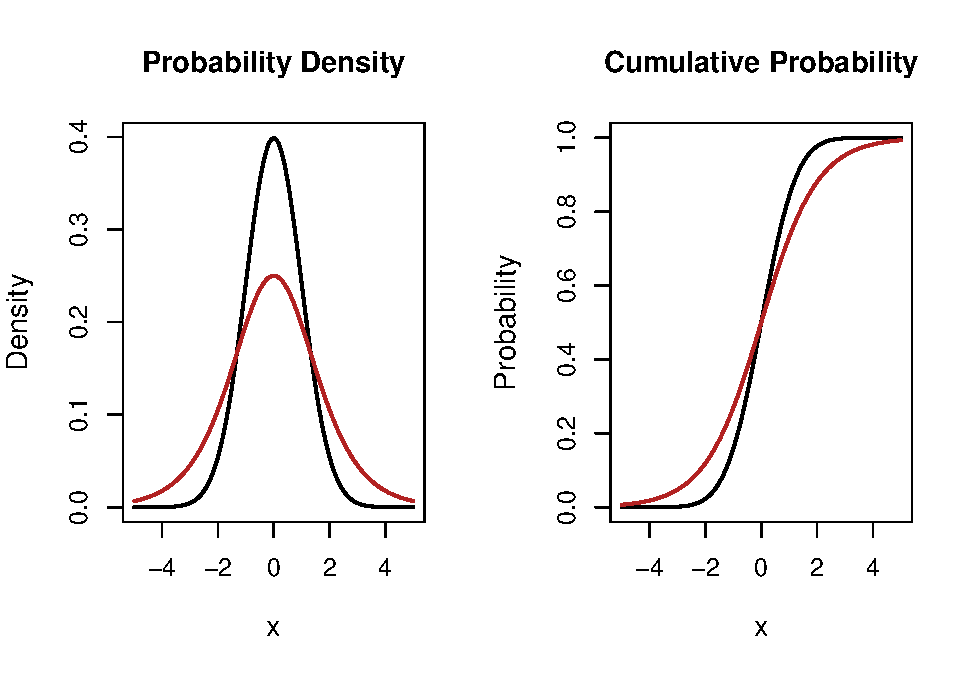
\includegraphics{paper-new_files/figure-latex/logit-vs-probit-1} 

}

\caption{Logit vs Probit}\label{fig:logit-vs-probit}
\end{figure}

Given the different underlying distribution, the parameters have a different interpretation under the two models. The probit model assume a latent standard normal distribution with and \(\sigma = 1\). The logit model assume a logistic distribution with \(\sigma^2 = \pi^2/3\). Thus regression coefficients \(\beta\) represents the increase in standard deviations units. The interpretation in terms of latent distribution is particularly useful for the probit model where \(\beta\)s can be interpreted in a Cohen's \(d\) like manner. Furthermore, there is the possibility to directly map parameters from signal detection theory (Green, Swets, \& Others, 1966; Stanislaw \& Todorov, 1999) into an ordinal probit regression. In practical terms, the thresholds are the criterion cut-offs and the \(\beta_1\) is the d\('\) parameter (DeCarlo, 1998; Knoblauch \& Maloney, 2012).

\subsection{Simulating data}\label{simulating-data}

There are mainly two ways to simulate data. The first method concerns simulating starting from the latent formulation of the ordinal model. Basically we can simulate the underlying latent distribution and then fixing the thresholds converting the latent continuous variable into the observed ordinal variable.

\begin{figure}

{\centering 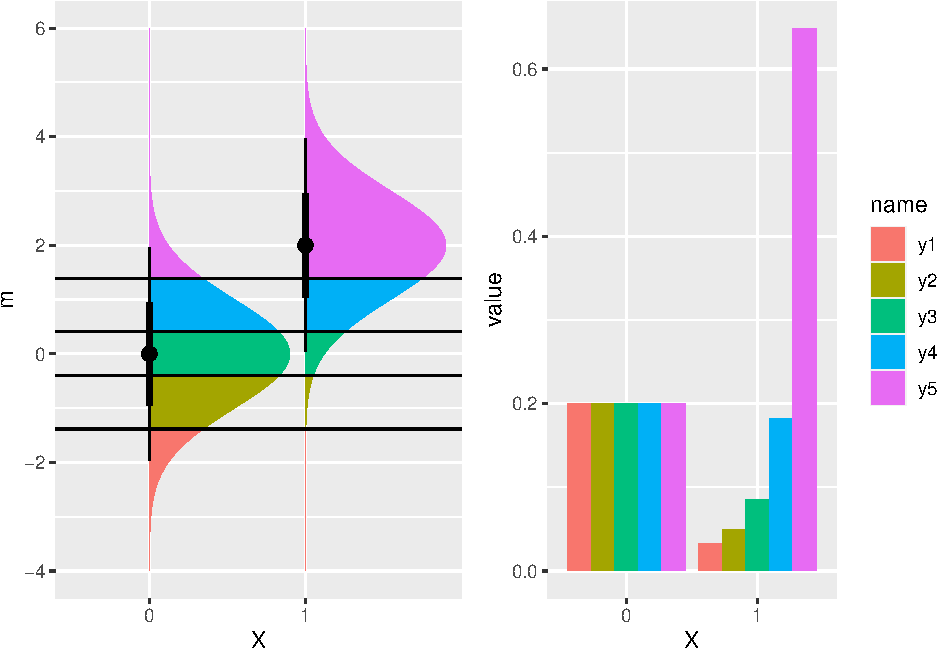
\includegraphics{paper-new_files/figure-latex/unnamed-chunk-3-1} 

}

\caption{ }\label{fig:unnamed-chunk-3}
\end{figure}

\newpage

\section{References}\label{references}

\phantomsection\label{refs}
\begin{CSLReferences}{1}{0}
\bibitem[\citeproctext]{ref-Cliff2016-ck}
Cliff, N. (2016). \emph{Ordinal methods for behavioral data analysis}. London, England: Psychology Press.

\bibitem[\citeproctext]{ref-DeCarlo1998-ay}
DeCarlo, L. T. (1998). Signal detection theory and generalized linear models. \emph{Psychological Methods}, \emph{3}, 186--205. \url{https://doi.org/10.1037/1082-989X.3.2.186}

\bibitem[\citeproctext]{ref-Green1966-gy}
Green, D. M., Swets, J. A., \& Others. (1966). \emph{Signal detection theory and psychophysics} (Vol. 1, pp. xi, 455--xi, 455). Oxford, England: Wiley New York.

\bibitem[\citeproctext]{ref-Kemp2021-dj}
Kemp, S., \& Grace, R. C. (2021). Using ordinal scales in psychology. \emph{Methods in Psychology (Online)}, \emph{5}, 100054. \url{https://doi.org/10.1016/j.metip.2021.100054}

\bibitem[\citeproctext]{ref-Knoblauch2012-to}
Knoblauch, K., \& Maloney, L. T. (2012). \emph{Modeling psychophysical data in r}. New York, NY: Springer New York. \url{https://doi.org/10.1007/978-1-4614-4475-6}

\bibitem[\citeproctext]{ref-Liddell2018-wu}
Liddell, T. M., \& Kruschke, J. K. (2018). Analyzing ordinal data with metric models: What could possibly go wrong? \emph{Journal of Experimental Social Psychology}, \emph{79}, 328--348. \url{https://doi.org/10.1016/j.jesp.2018.08.009}

\bibitem[\citeproctext]{ref-McCullagh1980-cw}
McCullagh, P. (1980). Regression models for ordinal data. \emph{Journal of the Royal Statistical Society}, \emph{42}, 109--127. \url{https://doi.org/10.1111/j.2517-6161.1980.tb01109.x}

\bibitem[\citeproctext]{ref-Robitzsch2020-la}
Robitzsch, A. (2020). Why ordinal variables can (almost) always be treated as continuous variables: Clarifying assumptions of robust continuous and ordinal factor analysis estimation methods. \emph{Frontiers in Education}, \emph{5}, 589965. \url{https://doi.org/10.3389/feduc.2020.589965}

\bibitem[\citeproctext]{ref-Stanislaw1999-jr}
Stanislaw, H., \& Todorov, N. (1999). Calculation of signal detection theory measures. \emph{Behavior Research Methods, Instruments, \& Computers: A Journal of the Psychonomic Society, Inc}, \emph{31}, 137--149. \url{https://doi.org/10.3758/bf03207704}

\bibitem[\citeproctext]{ref-Tutz2022-dg}
Tutz, G. (2022). Ordinal regression: A review and a taxonomy of models. \emph{Wiley Interdisciplinary Reviews. Computational Statistics}, \emph{14}. \url{https://doi.org/10.1002/wics.1545}

\end{CSLReferences}


\end{document}
